%!TEX root = ../../dissertation.tex

\section{Tables and Figures}

\begin{table}
\caption{Benchmark parameter values.}
\tabcolsep=0.2in
\centering
\begin{tabular}{lrl}
\toprule
Parameter  &  Value  &  Comment \\
\midrule

%& \\
\multicolumn{3}{l}{\textit Preferences} \\
$\rho$   &  $-1$  & IES $= 1/(1-\rho) = 1/2$ \\
$\alpha$ &  $-9$ & RA $= 1-\alpha = 10$ \\ %, Bansal \& Yaron (2004, Table II) \\
$\beta$  &   0.98 &  \\

\multicolumn{3}{l}{\textit Armington aggregator}  \\
$\sigma$    &   0   &  Cobb-Douglas   \\
$\omega$    &  0.1  &  chosen to hit import share of 0.1  \\

\multicolumn{3}{l}{\textit Productivity growth  } \\
$\log g$  &  0.004   &  Tallarini (2000, Table 4) \\
$v^{1/2}$ & 0.015   &  Tallarini (2000, Table 4), rounded off \\
$ \varphi_v$ & 0.95 & Backus, Ferriere, and Zin (2015, Table 1) \\
$ \tau$   &  $0.74 \times 10^{-5}$  & makes $v$ three standard deviations from zero \\
$ \gamma$ & 0.1 & persistence of productivity difference \\
\bottomrule
\end{tabular}
\label{tab:benchmark}
\end{table}



% ****************************************************************************
\clearpage
\begin{figure}[htb]
\caption{Consumption frontiers.
Lines represent the frontier quantities of consumption given unit quantities of the intermediate goods.
The dashed black line has $\omega = 1/2$, making the two final goods the same.
For the others, we choose an import share of 0.1
and use (\ref{eq:share-calculation}) to adjust $\omega$ as we vary $\sigma$.
The elasticities of substitution noted in the figure are $1/(1-\sigma)$.}

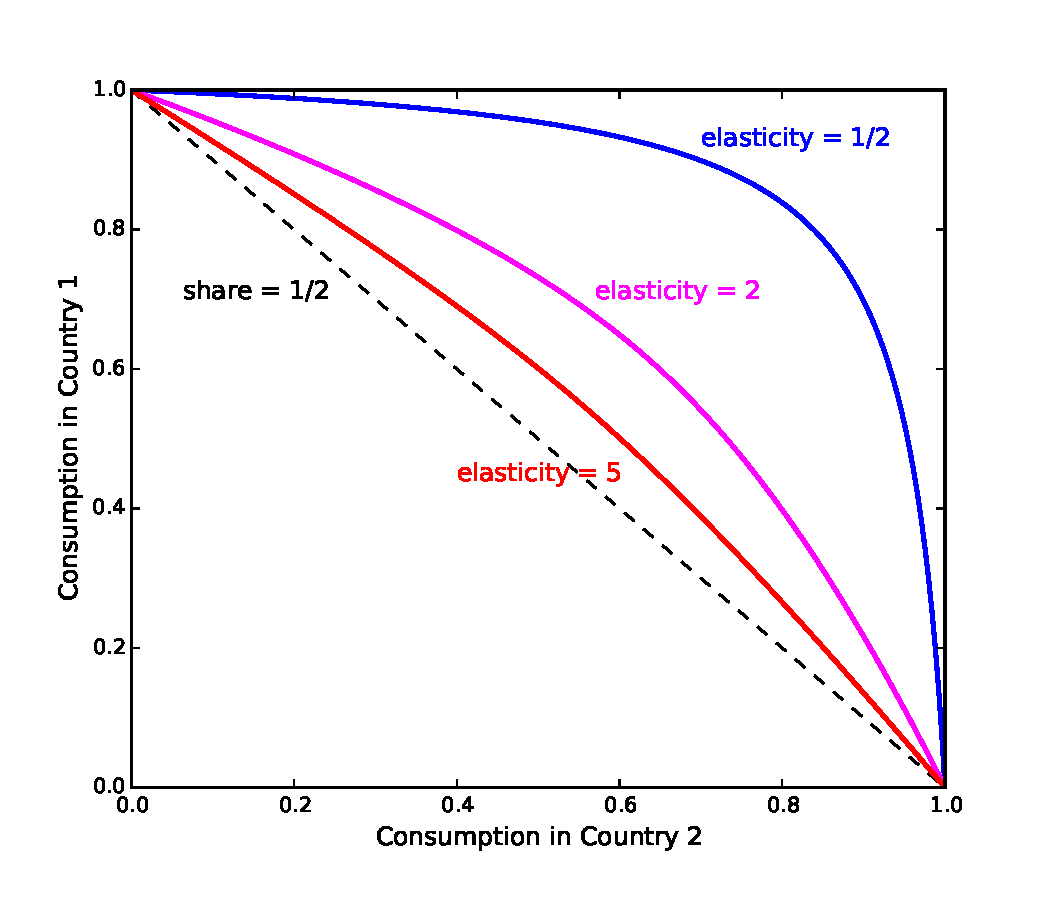
\includegraphics[width=\textwidth]{images/BCFL/final-goods-frontier.pdf}
\label{fig:consumption-frontier}
\end{figure}


% ****************************************************************************
\clearpage
\begin{figure}[htb]
\caption{Pareto and consumption frontiers.
The outer line is the consumption frontier with benchmark parameter values.
The inner line is the Pareto frontier:  the utility $J$ of agent 1 given
promised utility $U$ to agent 2.
In each case, the other state variables are $z_{1t} = z_{2t} = \wh{z}_t = 1$
and $v_t = v$.}

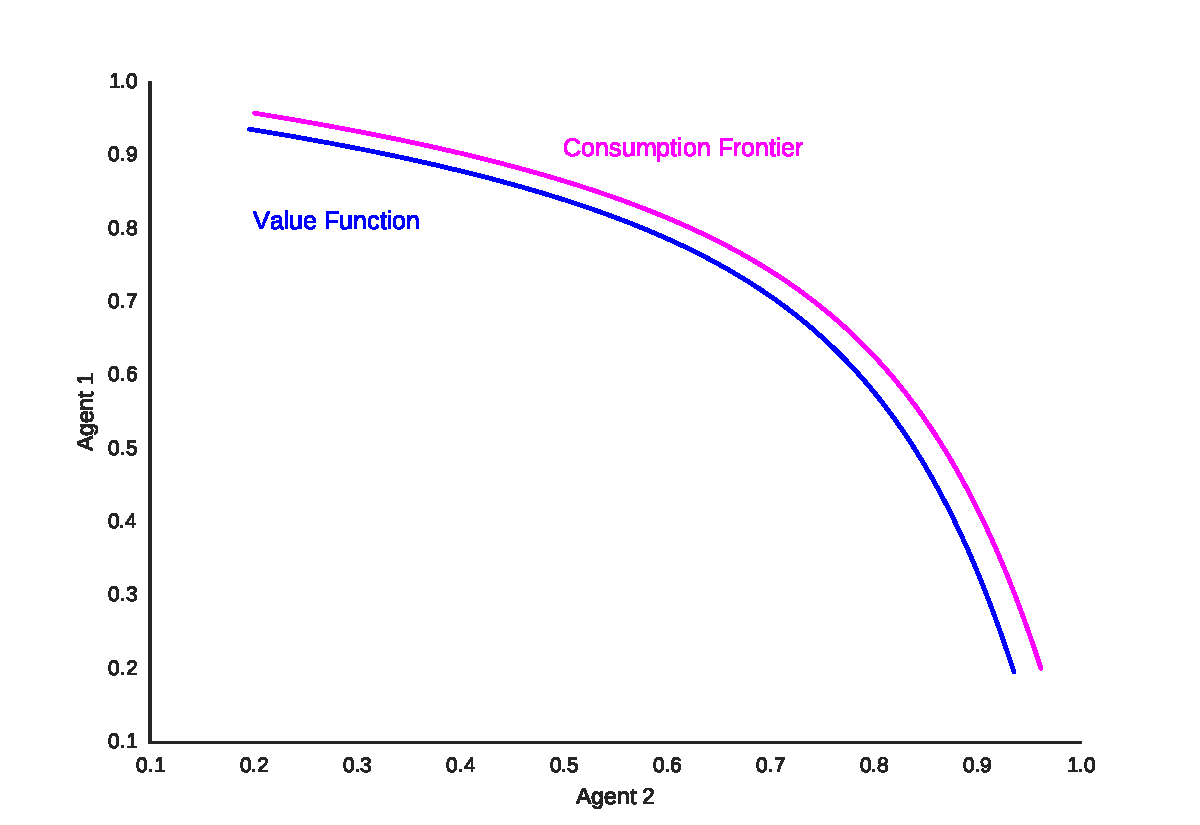
\includegraphics[width=\textwidth]{images/BCFL/frontiers_alpha9.pdf}
\label{fig:pareto-frontier}
\end{figure}


% ****************************************************************************
\clearpage
\begin{figure}[htb]
\caption{Dynamics of the additive and recursive Pareto weight.
The two lines represent simulations of models with additive ($\alpha = \rho = -1$)
and recursive ($\alpha = -9$, $\rho = -1 $) preferences.
The simulations use the same paths for exogenous state variables.
In each case, we plot $\log \lambda_t^*$ against time. }

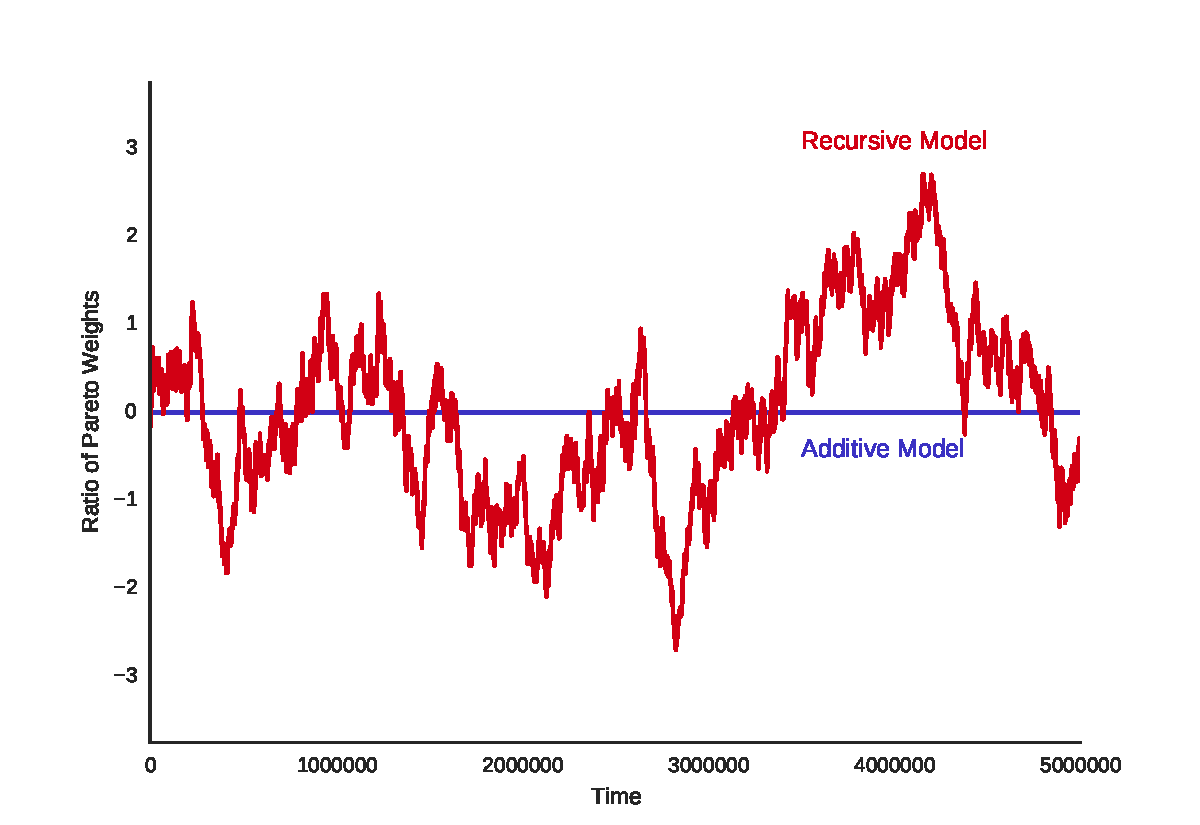
\includegraphics[width=\textwidth]{images/BCFL/paretoweightstability_alpha9.pdf}
\label{fig:exchange-pareto-weight-two}
\end{figure}


% ****************************************************************************
\clearpage
\begin{figure}[htb]
\caption{Risk aversion and expected changes in the Pareto weight.
The lines represent the expected change in $\log \lambda_t^*$, or $E_t[\log \lambda^*_{t+1}] - \log \lambda_t$,
with three values of risk aversion $1-\alpha$:
$2$ (additive), 10, and 50. }

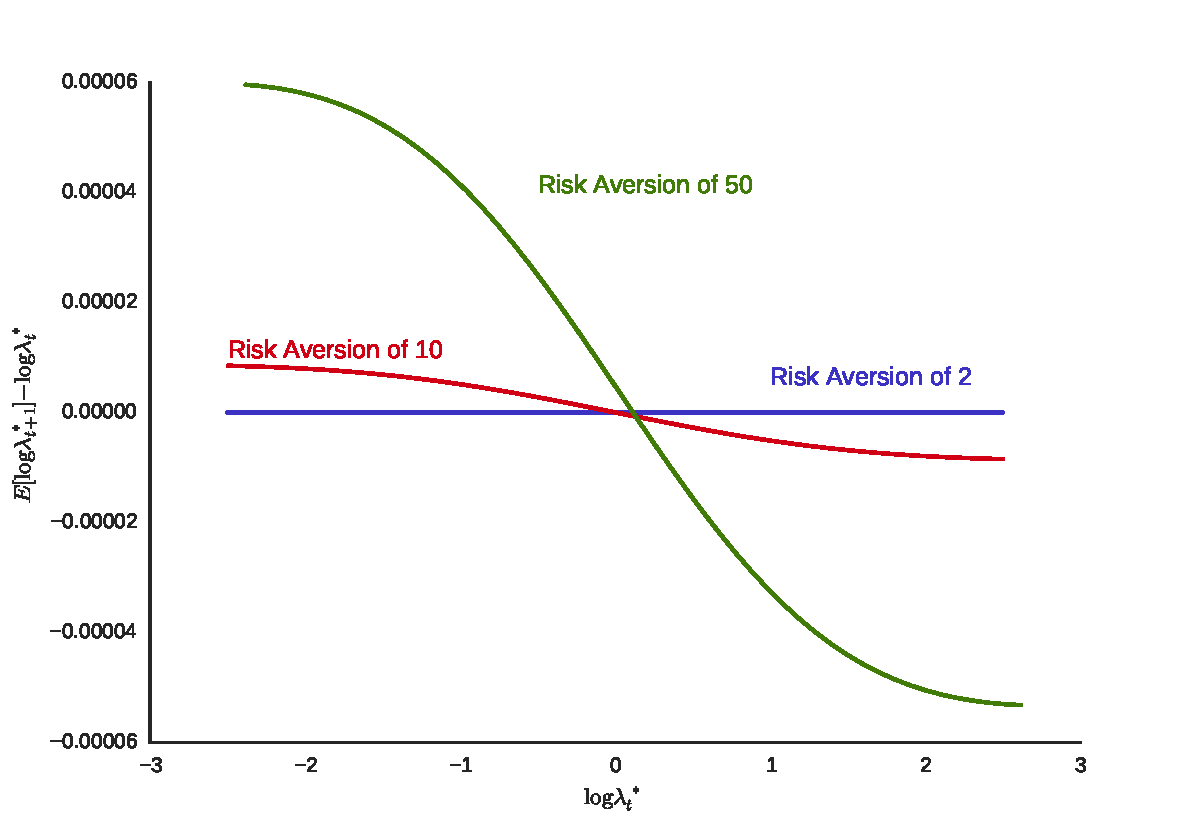
\includegraphics[width=\textwidth]{images/BCFL/policy_at_ss_one_axis.pdf}
\label{fig:change-pareto-weight-ra}
\end{figure}


% ****************************************************************************
\clearpage
\begin{figure}[htb]
\caption{Armington substitutability and expected changes in the Pareto weight.
The lines represent the expected change in $\log \lambda_t^*$, or $E_t[\log \lambda^*_{t+1}] - \log \lambda_t$,
with three values of the substitutability parameter $\sigma$ in the Armington aggregator.
The elasticities $1/(1-\sigma)$ are 2/3, 1, and 2. }

\bigskip
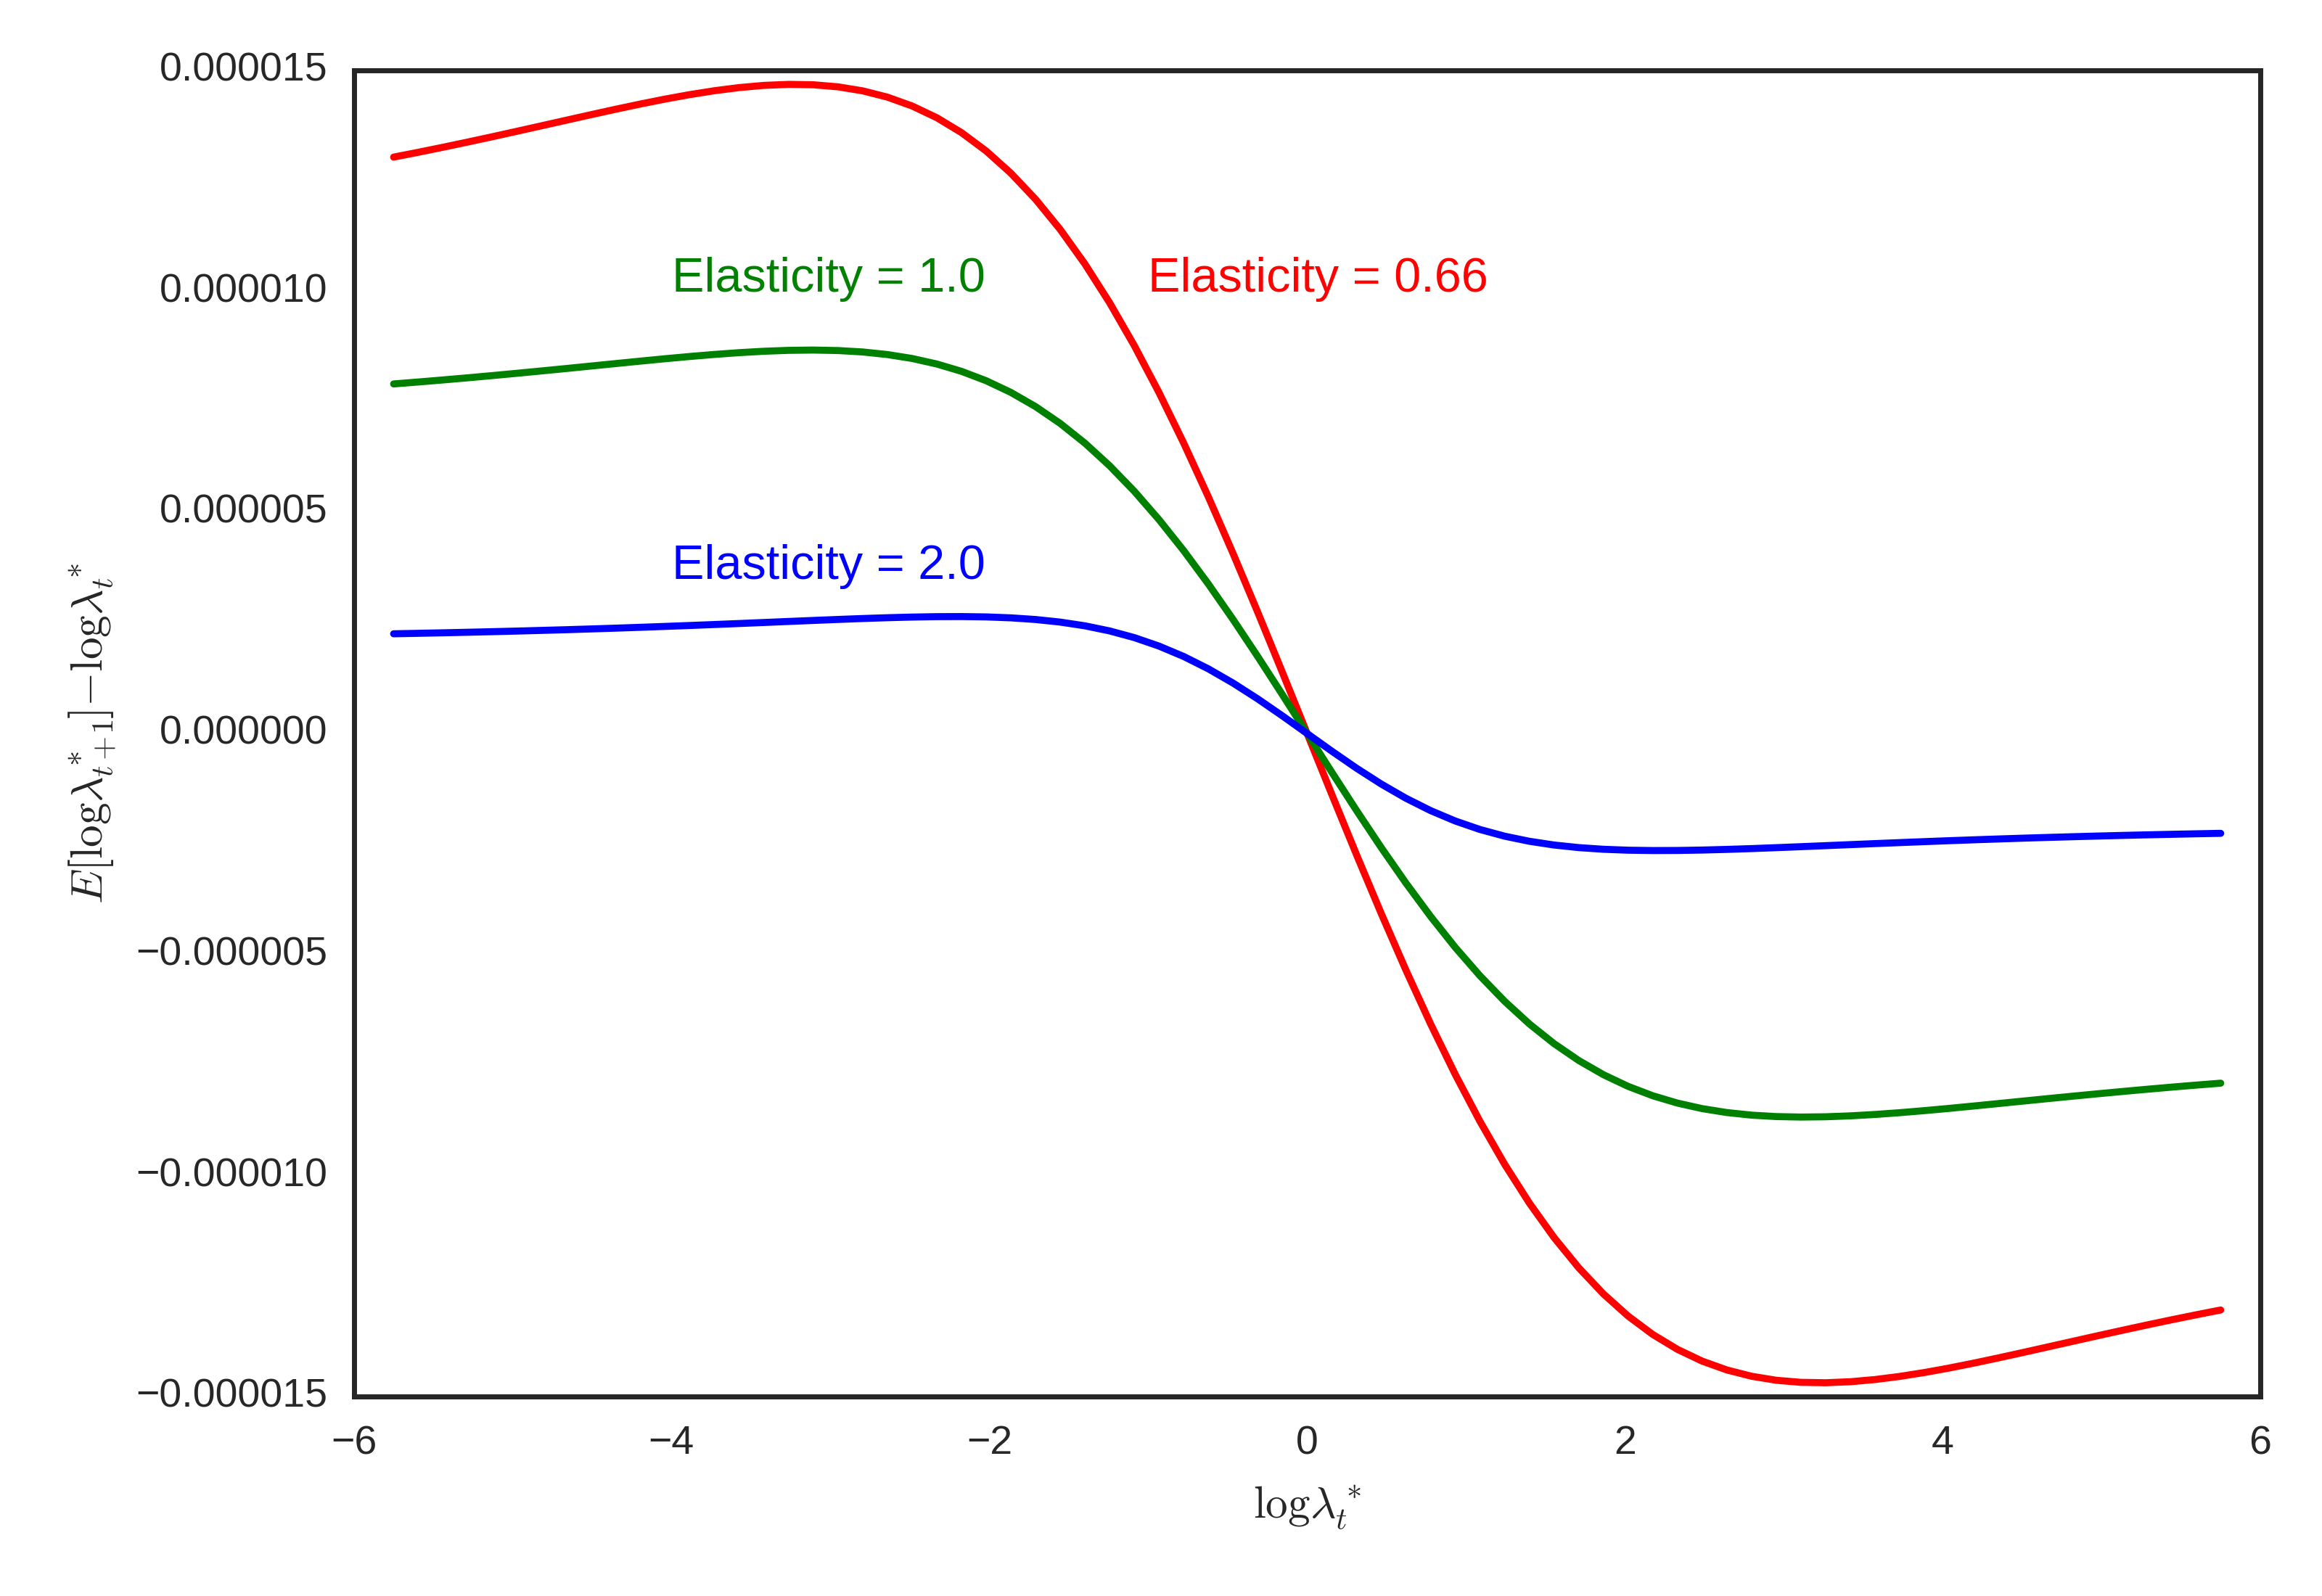
\includegraphics[width=\textwidth]{images/BCFL/Policies_Diff_Elast.png}
\label{fig:change-pareto-weight-arm}
\end{figure}

% ****************************************************************************
\clearpage
\begin{figure}[htb]
\caption{Intertemporal substitution and expected changes in the Pareto weight.
The lines represent the expected change in $\log \lambda_t^*$, or $E_t[\log \lambda^*_{t+1}] - \log \lambda_t$,
with three values of the substitutability parameter $\rho$ in the time aggregator:
$-1$, $-0.01$, and 1/3.
They correspond to intertemporal elasticities of substitution of 1/2, 0.99, and 3/2. }

\bigskip
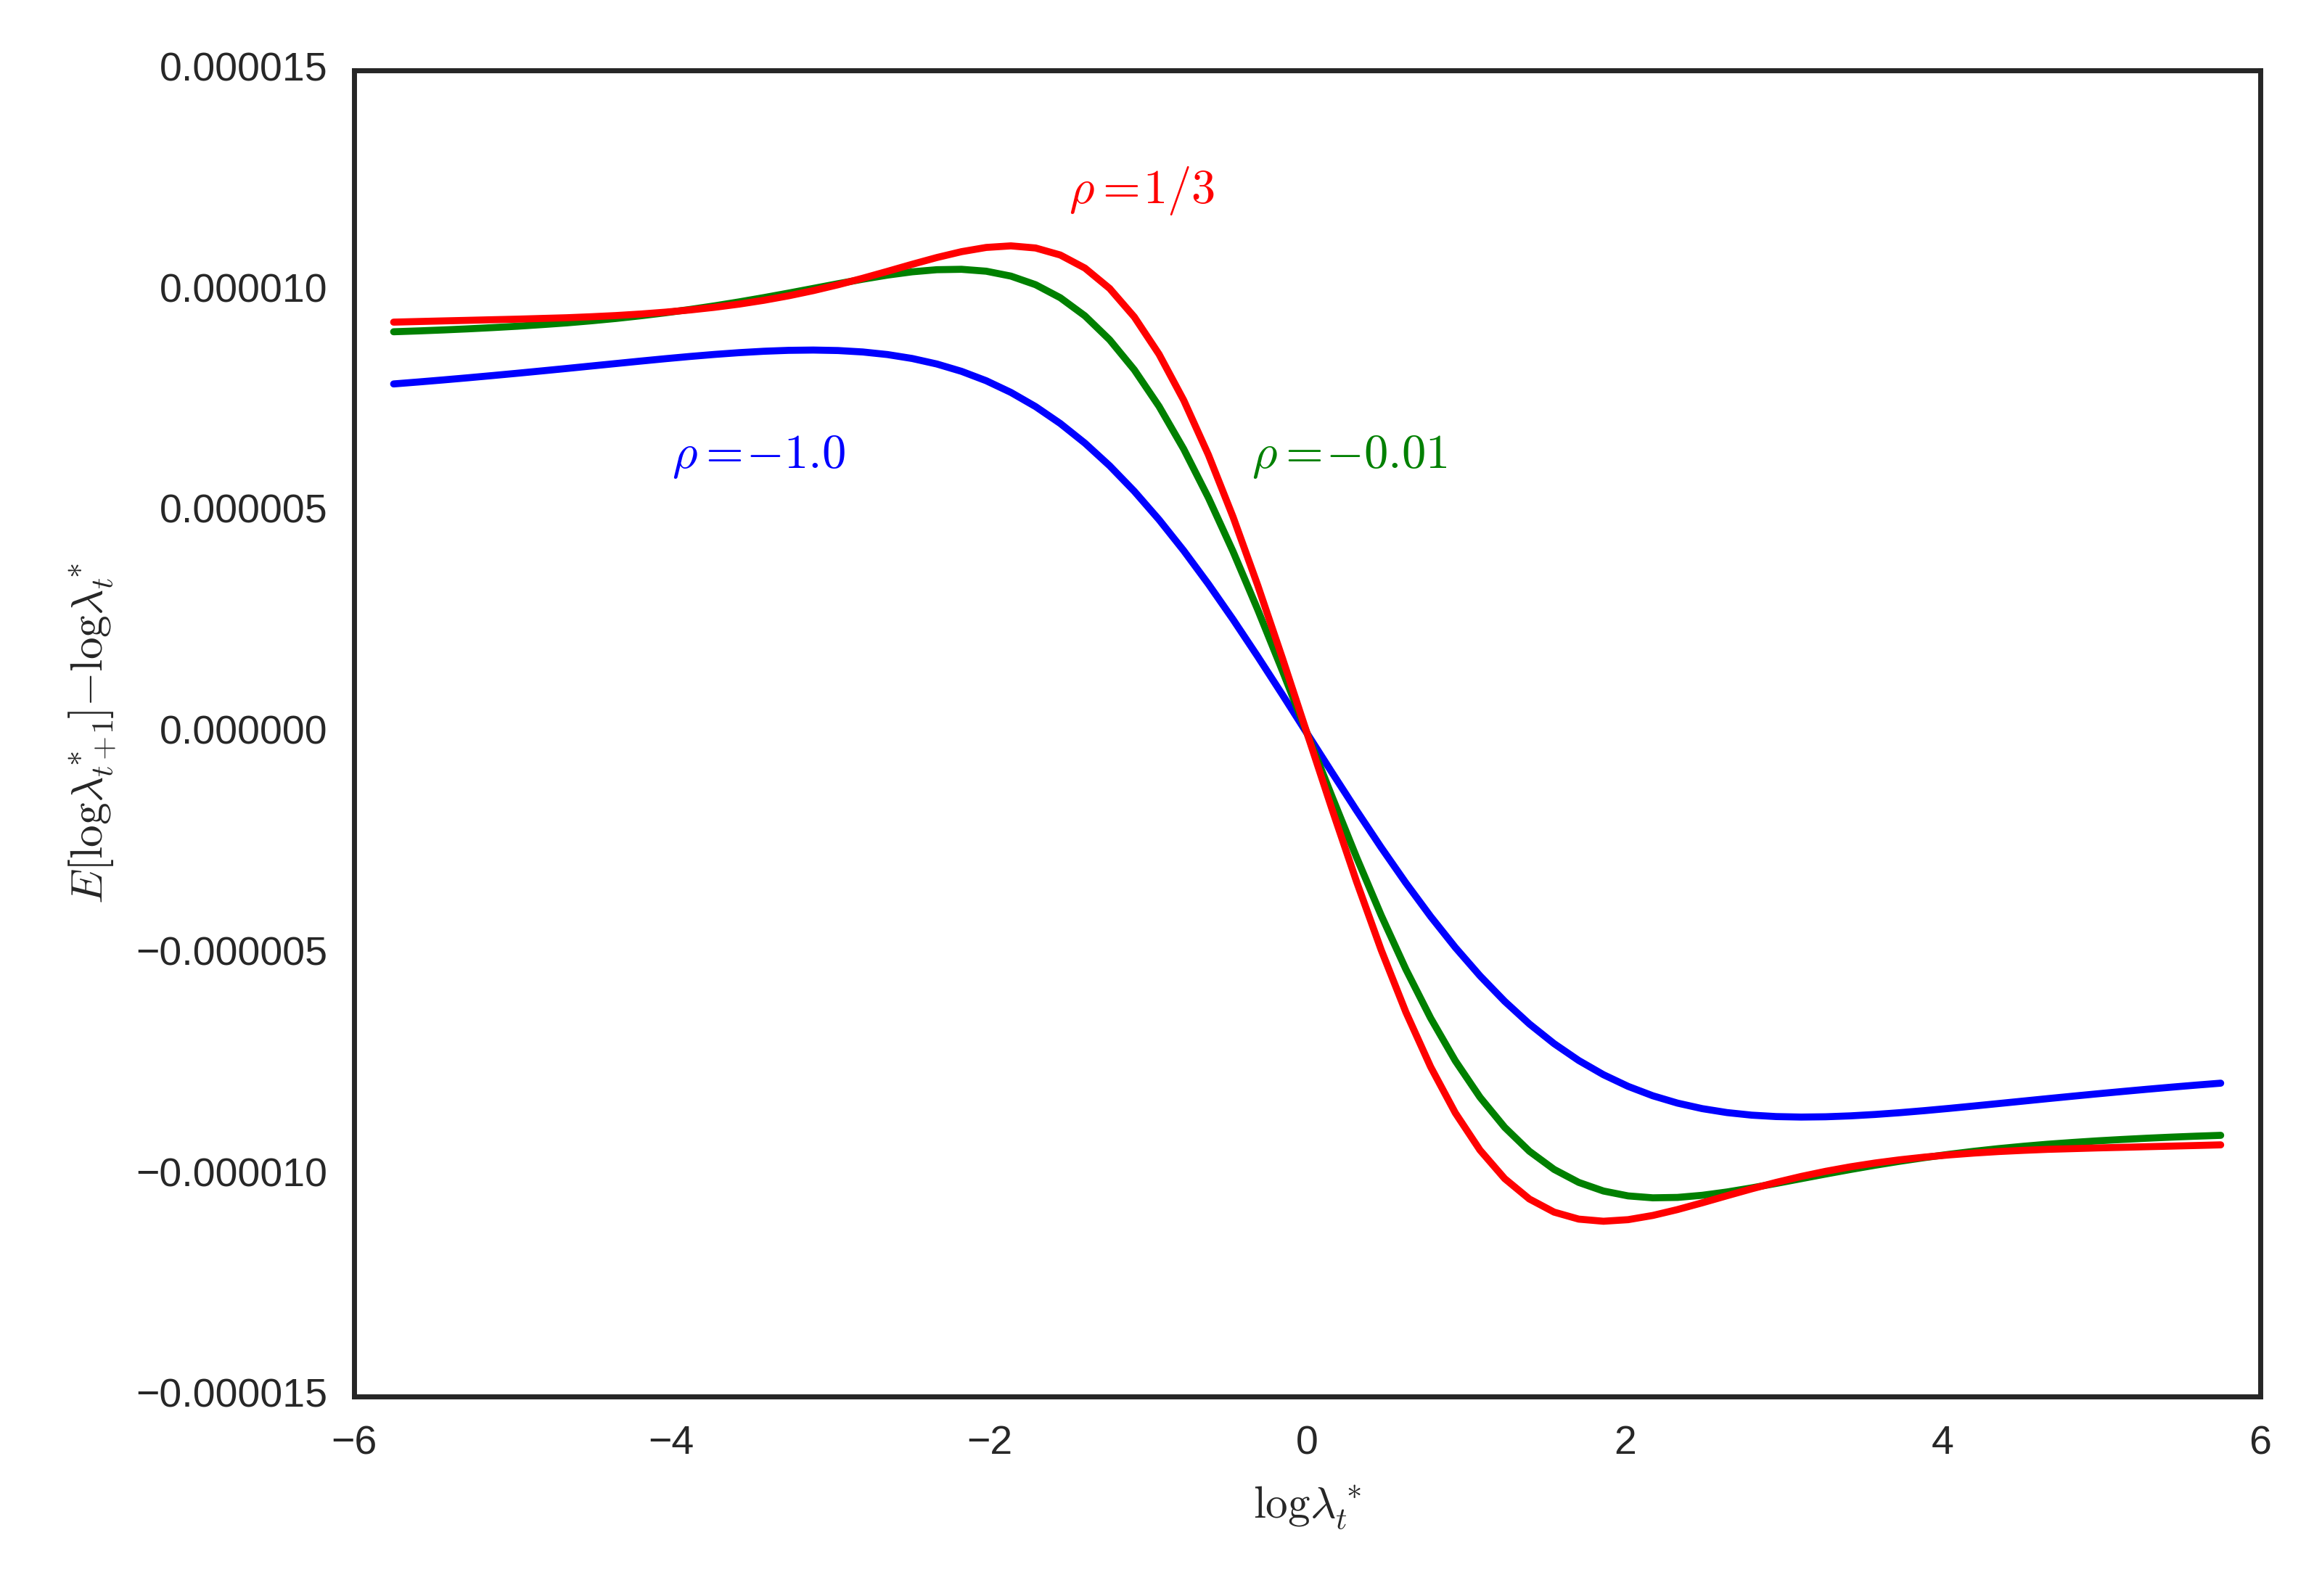
\includegraphics[width=\textwidth]{images/BCFL/Policies_Diff_rho.png}
\label{fig:change-pareto-weight-ies}
\end{figure}


% ****************************************************************************
\clearpage
\begin{figure}[htb]
\caption{Consumption and the real exchange rate.
The dots represent simulations of models with additive ($\alpha = \rho = -1$)
and recursive ($\alpha = -9$) preferences.
In each case, we plot  $\log e_t = \log (p_{2t}/p_{1t}) $ against $\log (c_{2t}/c_{1t}) $
for a simulation of the model. }

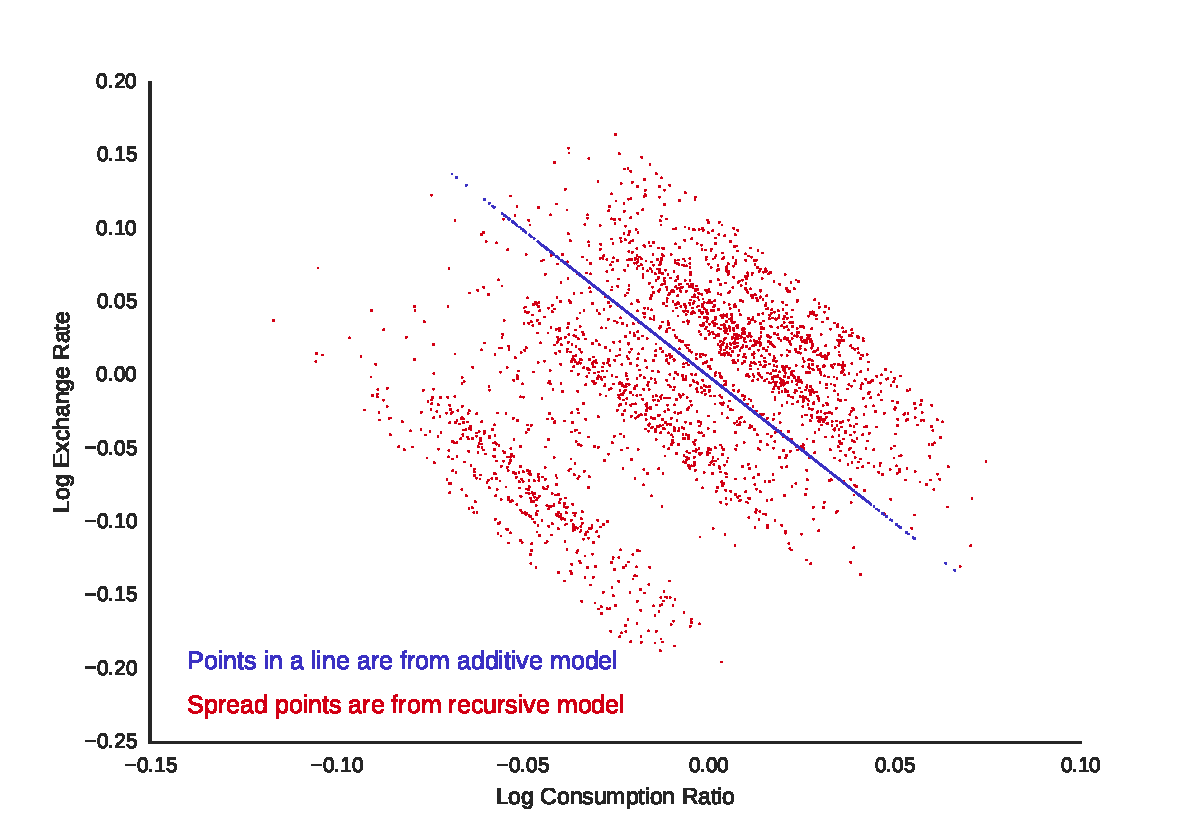
\includegraphics[width=\textwidth]{images/BCFL/con_v_fxr_alpha9.pdf}
\label{fig:exchange-cons-rer-two}
\end{figure}

%\end{document}
% ****************************************************************************
\clearpage
\begin{figure}[htb]
\caption{Dynamics of the real exchange rate.
The lines represent autocorrelation functions for the real exchange rate
($\log e_t$) in models with additive ($\alpha = \rho = -1$)
and recursive ($\alpha = -9$) preferences.}

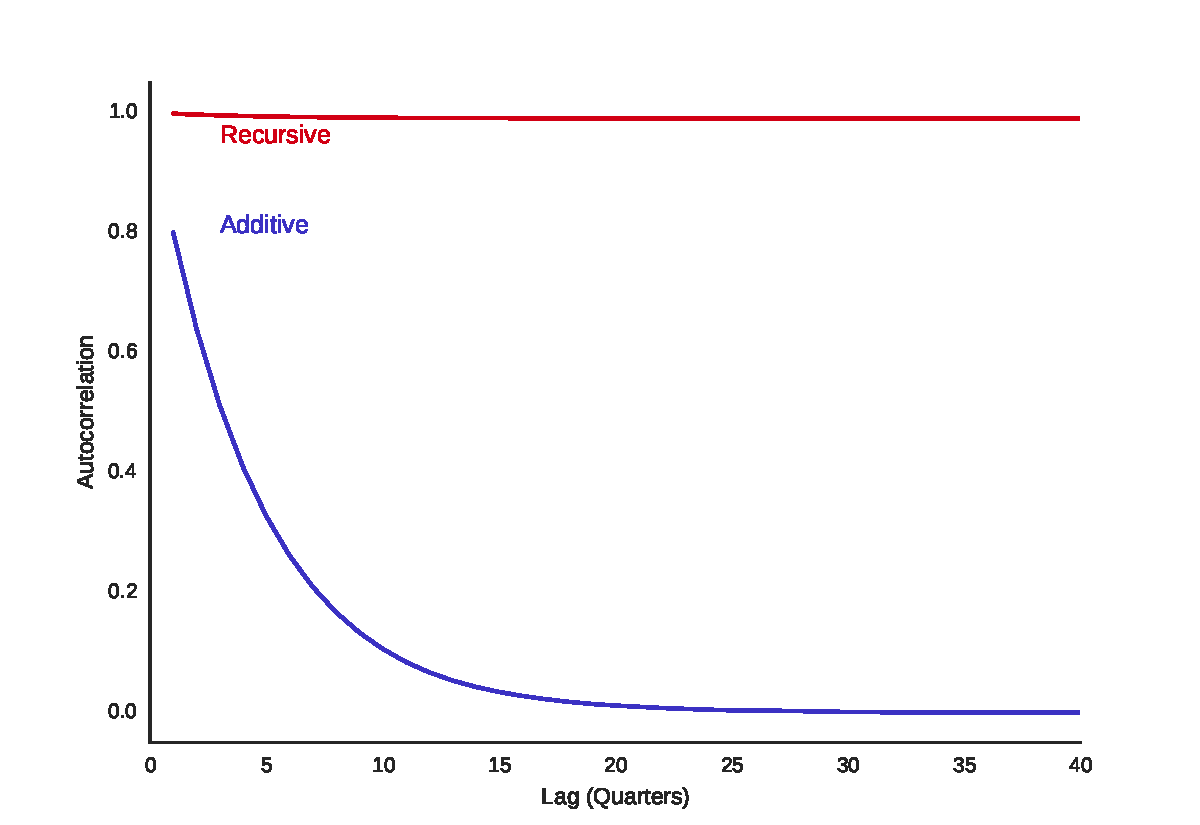
\includegraphics[width=\textwidth]{images/BCFL/acorr_fx_alpha1_9_one_axis.pdf}
\label{fig:rer-acfs}
\end{figure}

%\end{document}
% ****************************************************************************
\clearpage
\begin{figure}[htb]
\caption{Responses of variables
to an impulse in relative productivity\newline
$\log \wh{z}_t = (1/2) (\log z_{1t} - \log z_{2t}) $ in country 2.
The impulse takes place at date $t=1$.
Responses are reported as percent deviations from mean values.
}

\bigskip
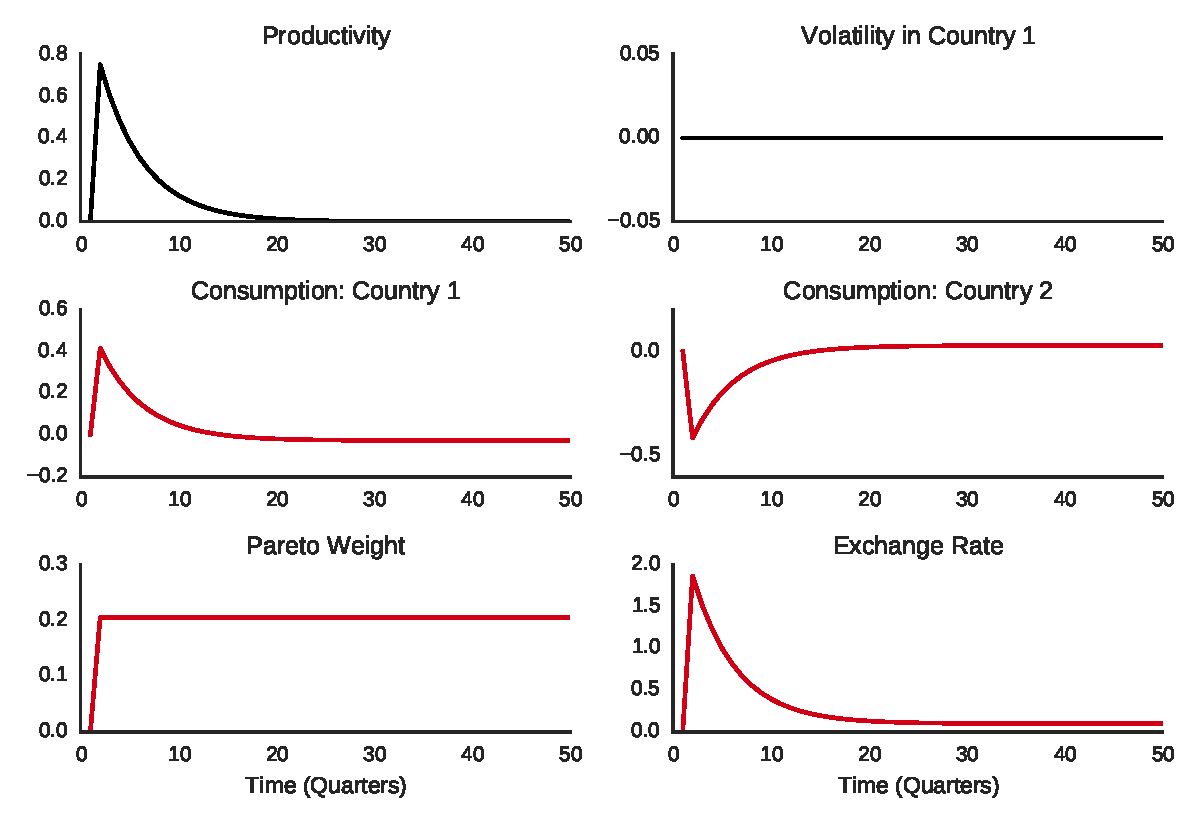
\includegraphics[width=\textwidth]{images/BCFL/irf_wrt_zhat_alpha9.pdf}
\label{fig:irf-zhat}
\end{figure}

%\end{document}
% ****************************************************************************
\clearpage
\begin{figure}[htb]
\caption{Responses of variables
to an impulse in volatility $v_t$.
The impulse takes place at date $t=1$.
Responses are reported as percent deviations from mean values.
}

\bigskip
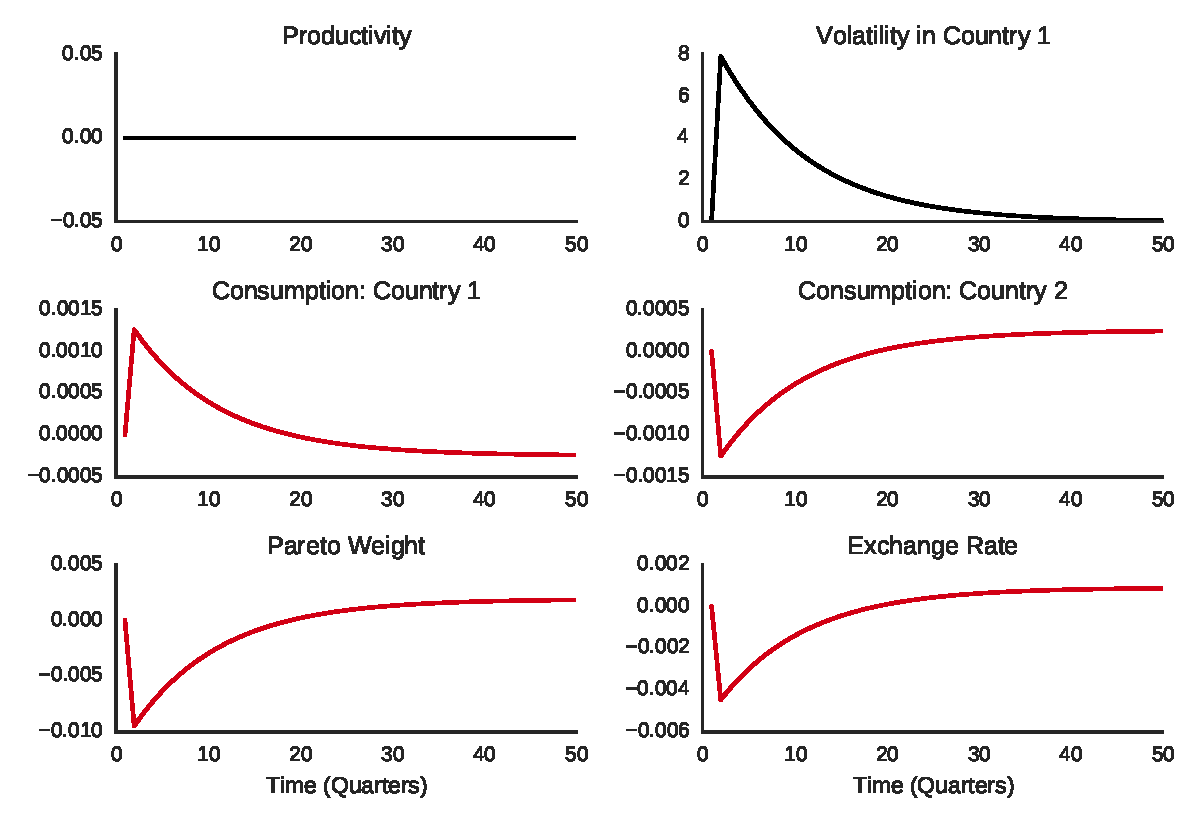
\includegraphics[width=\textwidth]{images/BCFL/irf_wrt_v_alpha9.pdf}
\label{fig:irf-v}
\end{figure}
